
%usepackage es egyebek
\input{common/globdef.tex}

%zarojel, FA...
% ez valahol kellett
\DeclarePairedDelimiter\ceil{\lceil}{\rceil}
\DeclarePairedDelimiter\floor{\lfloor}{\rfloor}

% zárójelek stb.
\newcommand{\Gzjel}[1]{%
{ \left( #1 \right) }
}

\newcommand{\gzjel}[1]{%
{ \left( #1 \right) }
}

\newcommand{\Toligv}[2]{%
#1,\hdots ,#2
}

\newcommand{\GZJ}[1]{%
{ \left( #1 \right) }
}

\newcommand{\KZJ}[1]{%
{ \{ #1 \} }
}

\newcommand{\SZZJ}[1]{%
{ \left[ #1 \right] }
}

\newcommand{\Tolig}[2]{%
#1\hdots #2
}

\newcommand{\SZOR}[2]{%
#1\cdot\hdots\cdot #2
}

% integrál rendes d-vel
\newcommand{\mint}[2]{%
\int #1 \text{d}#2
}

\newcommand{\mder}[2]{%
\frac{\text{d} #1}{\text{d}#2}
}


% ez máshogy van alapban
\newcommand{\tg}[0]{%
\text{tg}
}
\newcommand{\ctg}[0]{%
\text{ctg}
}



% rövidítések
\input{common/szavakdef.tex}

% tcolorbox-al kapcsolatos
\newcommand{\feher}[1]{%
\begin{tcolorbox}[colback=white]
#1
\end{tcolorbox}
}

\newcommand{\zold}[1]{%
\begin{tcolorbox}[colback=green!17]
#1
\end{tcolorbox}
}

\newcommand{\szurke}[1]{%
\begin{tcolorbox}[colback=gray!10!white]
#1
\end{tcolorbox}
}

\newcommand{\szurkeM}[1]{%
\begin{tcolorbox}[colback=gray!10!white, top=-5mm, bottom=3mm]
\begin{gather*}
#1
\end{gather*}
\end{tcolorbox}
}


\newcommand{\sarga}[1]{%
\begin{tcolorbox}[colback=yellow!10!white]
#1
\end{tcolorbox}
}

\newcommand{\barna}[1]{%
\begin{tcolorbox}[colback=brown!20!white]
#1
\end{tcolorbox}
}

\newcommand{\kek}[1]{%
\begin{tcolorbox}[colback=blue!20!white]
#1
\end{tcolorbox}
}

\newcommand{\Fa}[1]{%
\begin{tcolorbox}[colback=brown!20!white]
#1
\end{tcolorbox}
}

\newcommand{\Fnew}[0]{%
\end{tcolorbox}
\begin{tcolorbox}[colback=brown!20!white]
}




\newcommand{\Mo}[1]{%
\begin{tcolorbox}[colback=green!17]
#1
\end{tcolorbox}
}


\newcommand{\Mnew}[0]{%
\end{tcolorbox}
\begin{tcolorbox}[colback=green!17]
}


\newcommand{\egy}[1]{%
\Fa{\input{#1Fa}}
\Mo{\input{#1Mo}}
}


\definecolor{light-gray}{gray}{0.95}
\newcommand{\mcode}[1]{
   \colorbox{light-gray}{\texttt{#1}}
}


\begin{document}\begin{spacing}{1.2}

\section*{Nevezetes határértékek} \label{DB}
\nameref{DBe}
\newline
\nameref{DBnthroot}
\newline
\nameref{DBsin}
\newpage
\section*{az e-szám} \label{DBe}
\nameref{DBe1}
\vspace{0.5cm}
\LINK{
\hfill\nameref{DB}
}
\newpage
\section*{\mtit{Fa}alap} \label{DBe1}
\Fa{
\MatTag{ebase}{
   a_n=\gzjel{ 1+\frac{1}{n}}^{n} \hspace{0.5cm} \nearrow\\
   b_n=\gzjel{ 1+\frac{1}{n}}^{n+1} \hspace{0.5cm} \searrow\\
   a_n < b_m\hspace{1cm} \forall n,m
}
Azaz:
\Mat{
   \exists \lim_{n\to \infty} \gzjel{ 1+\frac{1}{n}}^{n}=\mathrm{e}
}

}
\vspace{0.5cm}
\LINK{
\nameref{DBe1Mo}
\hfill\nameref{DBe}
}
\newpage
\section*{\mtit{Mo}alap} \label{DBe1Mo}
\Mo{
A \amgm{}miatt:
\szurkeM{
   1\gzjel{ 1+\frac{1}{n}}^{n}<
   \gzjel{\frac{1 + 1+\frac{1}{n}+\cdots+1+\frac{1}{n}}{n+1}}^{n+1}=
   \gzjel{ 1+\frac{1}{n+1}}^{n+1}
}
az $a_n=\gzjel{1+\frac{1}{n}}^{n}$ \szigmon{}nő.


A \gmhm{}miatt:
\szurkeM{
   1\gzjel{ 1+\frac{1}{n}}^{n+1}>
   \gzjel{\frac{n+2}{1 + 1-\frac{1}{n+1}+\cdots+1-\frac{1}{n+1}}}^{n+2}=\\
   =\gzjel{ 1+\frac{1}{n+1}}^{n+2}
}
az $b_n=\gzjel{1+\frac{1}{n}}^{n+1}$ \szigmon{}csökken.
Könnyen látható, hogy:
\szurkeM{
   a_n < b_m \hspace{1cm} \forall m,n \\
   b_n-a_n=\frac{a_n}{n}
}
Mindezek miatt a sorozatok konvergensek és a határértékeik egybeesnek. Ezt
a számot $e$-vel szokták jelölni.

}
\vspace{0.5cm}
\LINK{
\nameref{DBe1}
\hfill\nameref{DBe}
}
\newpage
\section*{n-edik gyök} \label{DBnthroot}
\nameref{DBnthrootSum}
\newline
\nameref{DBnthroot1}
\newline
\nameref{DBnthroot2}
\newline
\nameref{DBnthroot2a}
\newline
\nameref{DBnthroot3}
\vspace{0.5cm}
\LINK{
\hfill\nameref{DB}
}
\newpage
\section*{\mtit{Fa}Létezés...} \label{DBnthrootSum}
\Fa{
\szurkeM{
   a,b\in \mathbb{R}, \ n\in\mathbb{N}\\
   \forall \ a>0, n>1 \ : \ \exists! \ b>0 \ : \ b^n=a \\
   \text{jele:}\ b=a^{\frac{1}{n}}
}
Tulajdonság:
\szurkeM{
   (a^{\frac{1}{n}})^m=(a^m)^\frac{1}{n}
}

}
\vspace{0.5cm}
\LINK{
\nameref{DBnthrootSumMo}
\hfill\nameref{DBnthroot}
}
\newpage
\section*{\mtit{Mo}Létezés...} \label{DBnthrootSumMo}
\Mo{
Legyen $a>1$ és
\szurkeM{
   a_{-}=\{ b\ :\ b^n < a \}\\
   a_{+}=\{ b\ :\ b^n > a \}
}
Megfigyelések:
\begin{itemize}
   \item $a_{-}$ és $a_{+}$ nemüresek
   \item bármely $b\in a_{+}$ felső korlátja $a_{-}$
   \item bármely $b\in a_{-}$ alsó korlátja $a_{+}$
\end{itemize}
A valós számok felső/alsó-határ tulajdonsága miatt egyértelműen létezik
$S=\sup a_{-}$ és $I=\inf a_{+}$ és $S\le I.$
Ha $S < I$ akkor az ábra segít megtalálni az ellentmondást:
\begin{center}
\frame{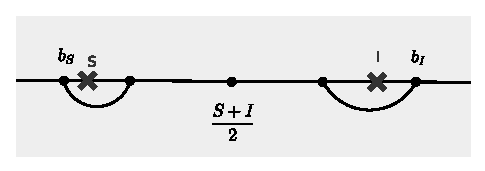
\includegraphics[scale=1.2]{DB/fig/nthroot}}
\end{center}
Tehát $S=I.$ Ezért: $I^n = S^n \le a$ és $I^n\ge a$, vagyis az $S=I$ szám
valóban $a^{\frac{1}{n}}$-ként viselkedik.
%!TODO!


}
\vspace{0.5cm}
\LINK{
\nameref{DBnthrootSum}
\hfill\nameref{DBnthroot}
}
\newpage
\section*{\mtit{Fa}konstans} \label{DBnthroot1}
\Fa{
\szurkeM{
   a^{\frac{1}{n}} \to 1 \hspace{1cm} a\in\mathbb{R}
}

}
\vspace{0.5cm}
\LINK{
\nameref{DBnthroot1Mo}
\hfill\nameref{DBnthroot}
}
\newpage
\section*{\mtit{Mo}konstans} \label{DBnthroot1Mo}
\Mo{
Legyen $a>1$, ekkor valamely $a_n>0$ sorozattal $a^{\frac{1}{n}}=1+a_n$.
A következő megállapításokat tehetjük:
\szurkeM{
   a=\gzjel{1+a_n}^n \ge 1+na_n \hspace{1cm}(\text{Bernoulli})\\
   \frac{a-1}{n}\ge a_n \\
   1\le a^{\frac{1}{n}}\le 1+\frac{a-1}{n}\hspace{1cm}(\text{rendőr-elv})
}
$a<1$ esetén alkalmazzuk $\frac{1}{a}$-ra a fentieket.

}
\vspace{0.5cm}
\LINK{
\nameref{DBnthroot1}
\hfill\nameref{DBnthroot}
}
\newpage
\section*{\mtit{Fa}$n$} \label{DBnthroot2}
\Fa{
\Mat{
   \gzjel{ 1-\frac{1}{n}}^{n}\nearrow \frac{1}{\mathrm{e}}\\
   \gzjel{ 1-\frac{1}{n+1}}^{n}\searrow \frac{1}{\mathrm{e}}
}

}
\vspace{0.5cm}
\LINK{
\nameref{DBnthroot2Mo}
\hfill\nameref{DBnthroot}
}
\newpage
\section*{\mtit{Mo}$n$} \label{DBnthroot2Mo}
\Mo{
A következő megállapításokat tehetjük:
\szurkeM{
   n=\gzjel{1+a_n}^n \ge 1+\frac{n(n-1)}{2}a^2_n \hspace{1cm}(\text{Binomiális})\\
   \sqrt{\frac{2}{n}}\ge a_n \\
   1\le n^{\frac{1}{n}}\le 1+\sqrt{\frac{2}{n}}\\\
   n^{\frac{1}{n}}\to 1 \hspace{1cm}(\text{rendőr-elv})
}

}
\vspace{0.5cm}
\LINK{
\nameref{DBnthroot2}
\hfill\nameref{DBnthroot}
}
\newpage
\section*{\mtit{Fa}polinom} \label{DBnthroot2a}
\Fa{
\szurkeM{
   a_0,\hdots,a_m>0\\
   P(n)=\sum_{k=0}^m a_k n^k \\
   P(n)^{\frac{1}{n}}\to 1
}

}
\vspace{0.5cm}
\LINK{
\nameref{DBnthroot2aMo}
\hfill\nameref{DBnthroot}
}
\newpage
\section*{\mtit{Mo}polinom} \label{DBnthroot2aMo}
\Mo{
Legyen $a=\max\{ a_0,\hdots,a_m \}$:
\szurkeM{
   a_m n^m \le P(n) \le (m+1)an^m \hspace{1cm} (\text{rendőr-elv})
}

}
\vspace{0.5cm}
\LINK{
\nameref{DBnthroot2a}
\hfill\nameref{DBnthroot}
}
\newpage
\section*{\mtit{Fa}$n!$} \label{DBnthroot3}
\Fa{
\szurkeM{
   (n!)^{\frac{1}{n}} \to \infty
}

}
\vspace{0.5cm}
\LINK{
\nameref{DBnthroot3Mo}
\hfill\nameref{DBnthroot}
}
\newpage
\section*{\mtit{Mo}$n!$} \label{DBnthroot3Mo}
\Mo{
A \amqm{}és egyszerű átalakítás mutatja:
\szurkeM{
   \gzjel{\frac{\sum{\frac{1}{k}}}{n}}^2\le
   \frac{\sum{\frac{1}{k^2}}}{n}\le
   \frac{\sum{\frac{2}{k(k+1)}}}{n}=
   2\frac{1-\frac{1}{n+1}}{n}\le\frac{2}{n}
}
A \gmhm{ből:}
\szurkeM{
   (n!)^{\frac{1}{n}} \ge \frac{n}{\sum\frac{1}{k}}\ge
   \sqrt{\frac{n}{2}}
}

}
\vspace{0.5cm}
\LINK{
\nameref{DBnthroot3}
\hfill\nameref{DBnthroot}
}
\newpage
\section*{$\frac{\sin(x)}{x}$ és környéke} \label{DBsin}
\nameref{DBsinSum}
\newline
\nameref{DBsin1}
\newline
\nameref{DBsin2}
\newline
\nameref{DBsin3}
\vspace{0.5cm}
\LINK{
\hfill\nameref{DB}
}
\newpage
\section*{\mtit{Desc}${\sin} -{\tan}$ lemma} \label{DBsinSum}
\Desc{
\MatTag{sin-tan}{
   \sin(x)< x < \tg(x) \hspace{1cm} -\frac{\pi}{2}<x<\frac{\pi}{2}
}
\egykep{sintan}
%~ \begin{center}
  %~ \makebox[\textwidth]{\includegraphics[width=\textwidth]{DB/fig/sintan}}
%~ \end{center}
%\frame{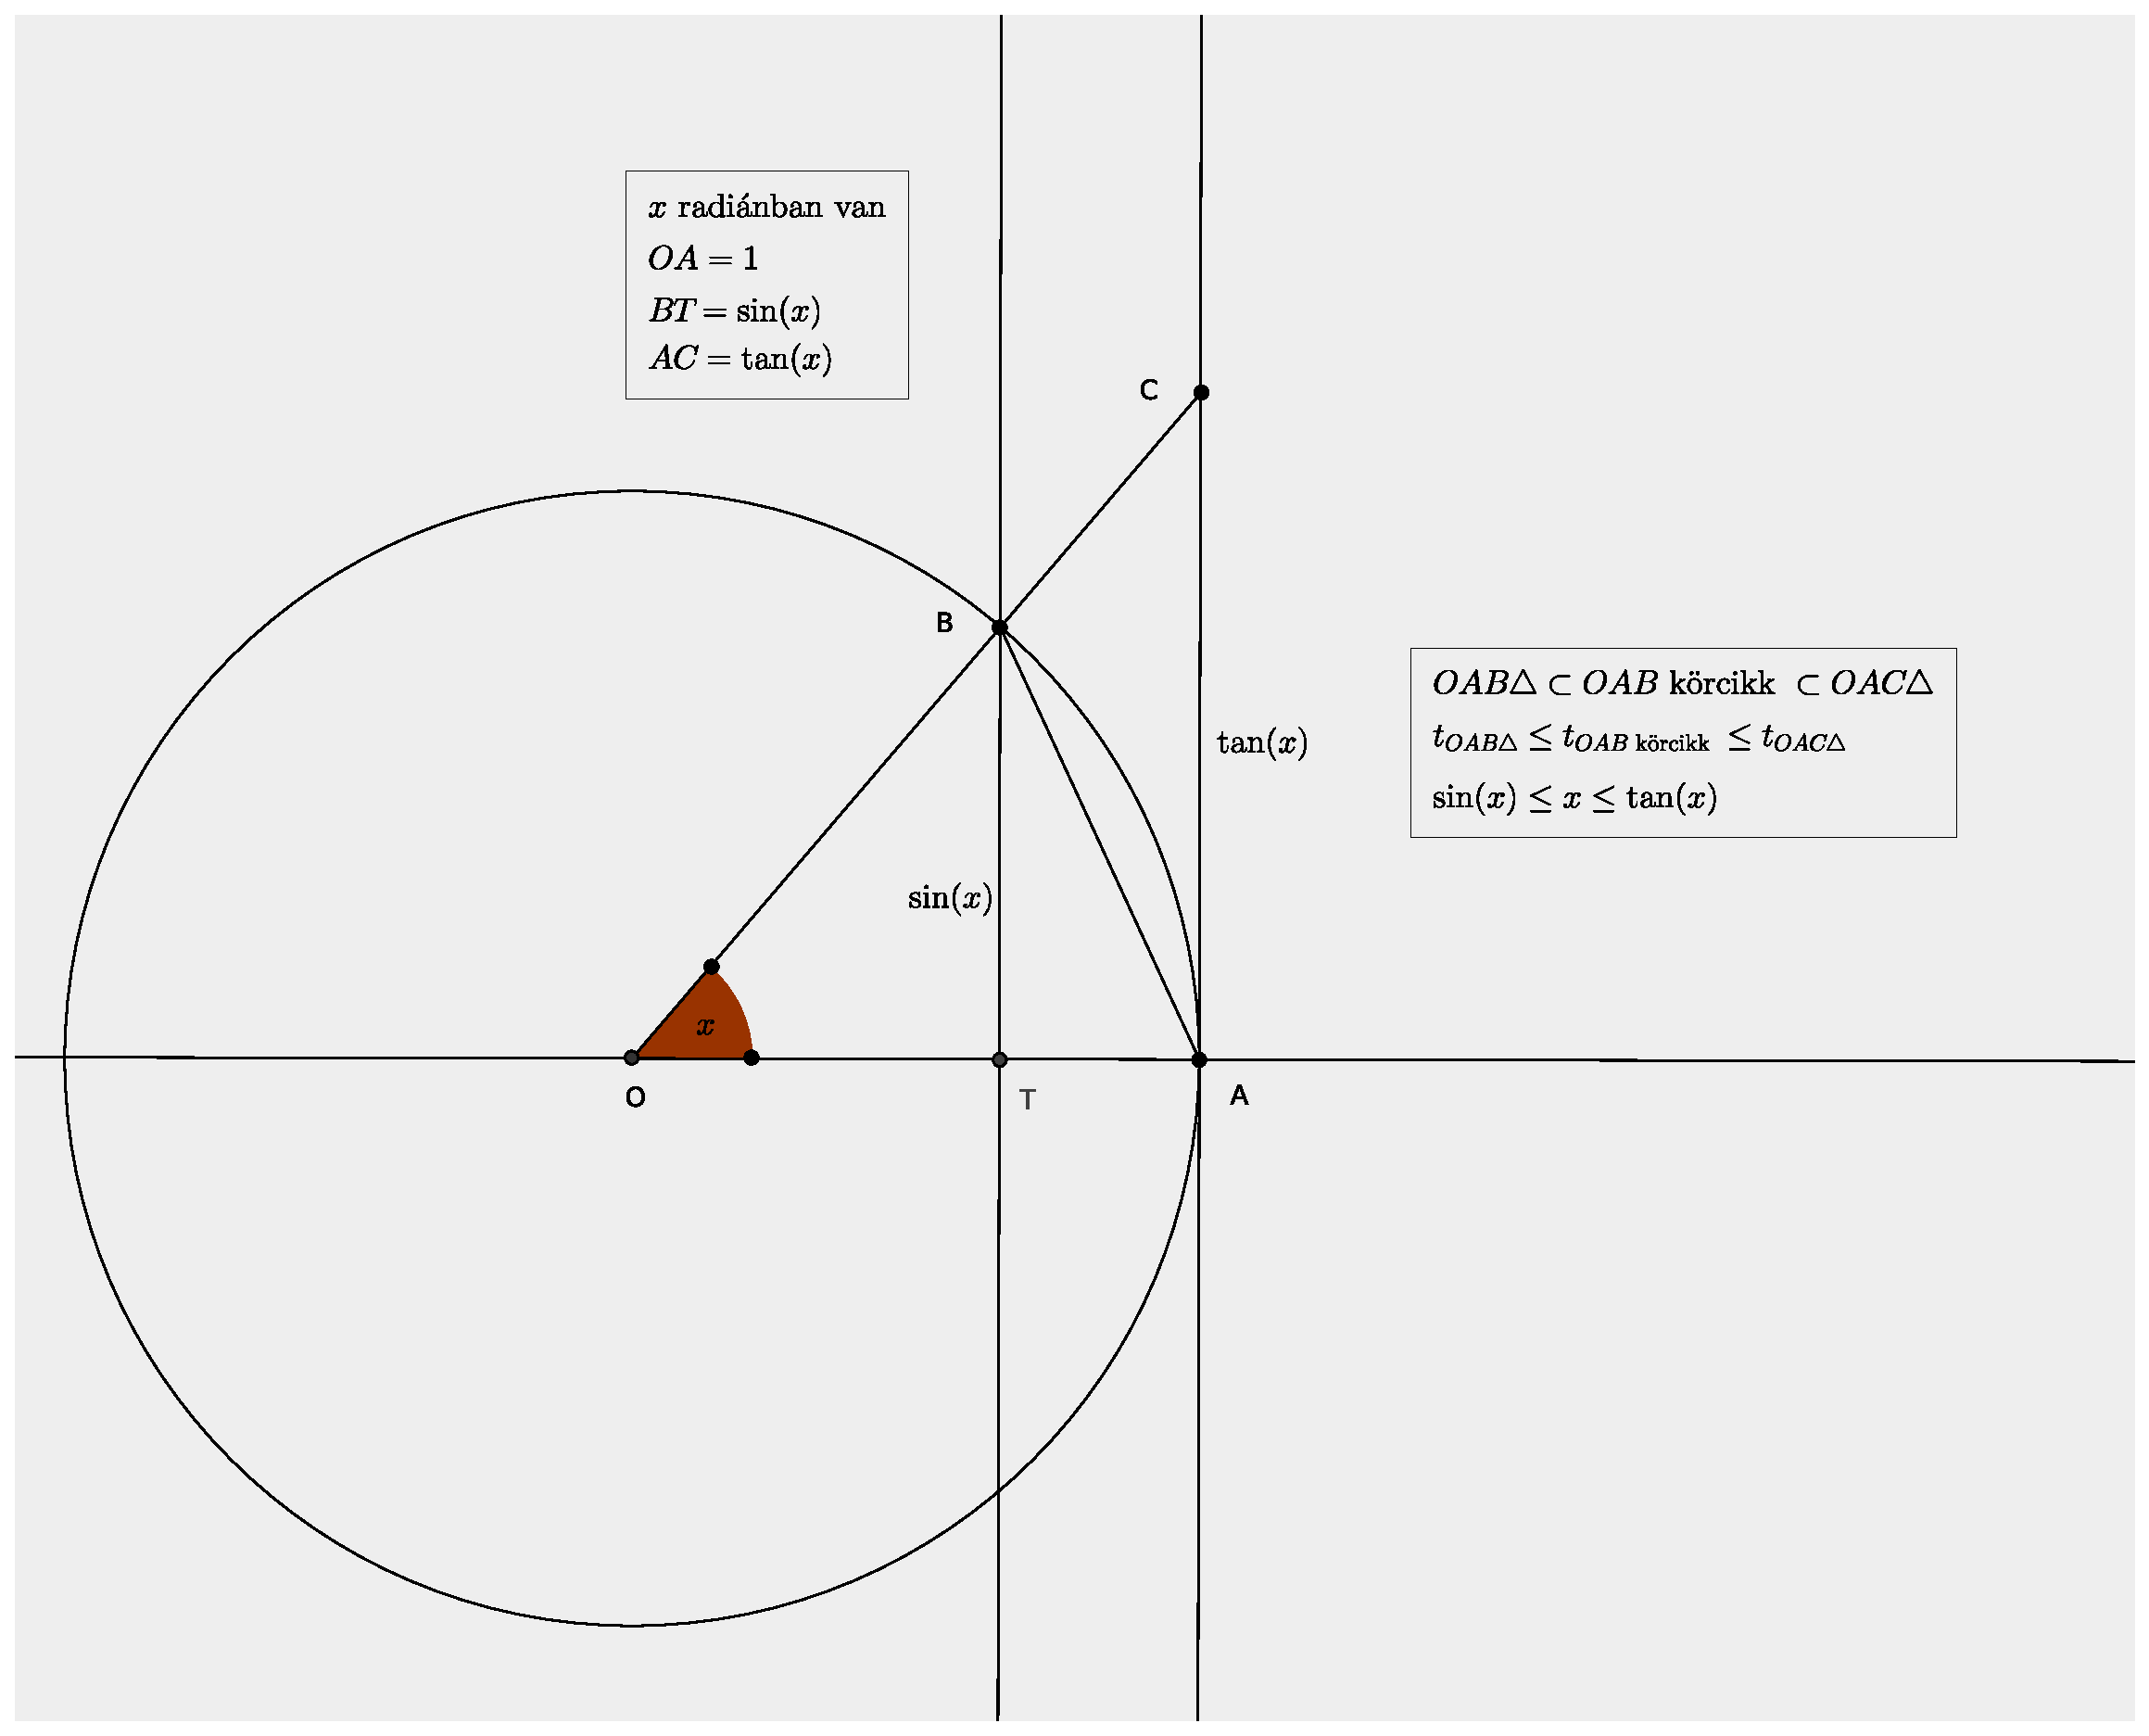
\includegraphics[scale=\textwidth]{DB/fig/sin}}

}
\vspace{0.5cm}
\LINK{
\hfill\nameref{DBsin}
}
\newpage
\section*{\mtit{Fa}$\frac{\sin(x)}{x}\to 1$} \label{DBsin1}
\Fa{
\MatTag{ebase}{
   a_n=\gzjel{ 1+\frac{1}{n}}^{n} \hspace{0.5cm} \nearrow\\
   b_n=\gzjel{ 1+\frac{1}{n}}^{n+1} \hspace{0.5cm} \searrow\\
   a_n < b_m\hspace{1cm} \forall n,m
}
Azaz:
\Mat{
   \exists \lim_{n\to \infty} \gzjel{ 1+\frac{1}{n}}^{n}=\mathrm{e}
}

}
\vspace{0.5cm}
\LINK{
\nameref{DBsin1Mo}
\hfill\nameref{DBsin}
}
\newpage
\section*{\mtit{Mo}$\frac{\sin(x)}{x}\to 1$} \label{DBsin1Mo}
\Mo{
%\begin{center}
%  \makebox[\textwidth]{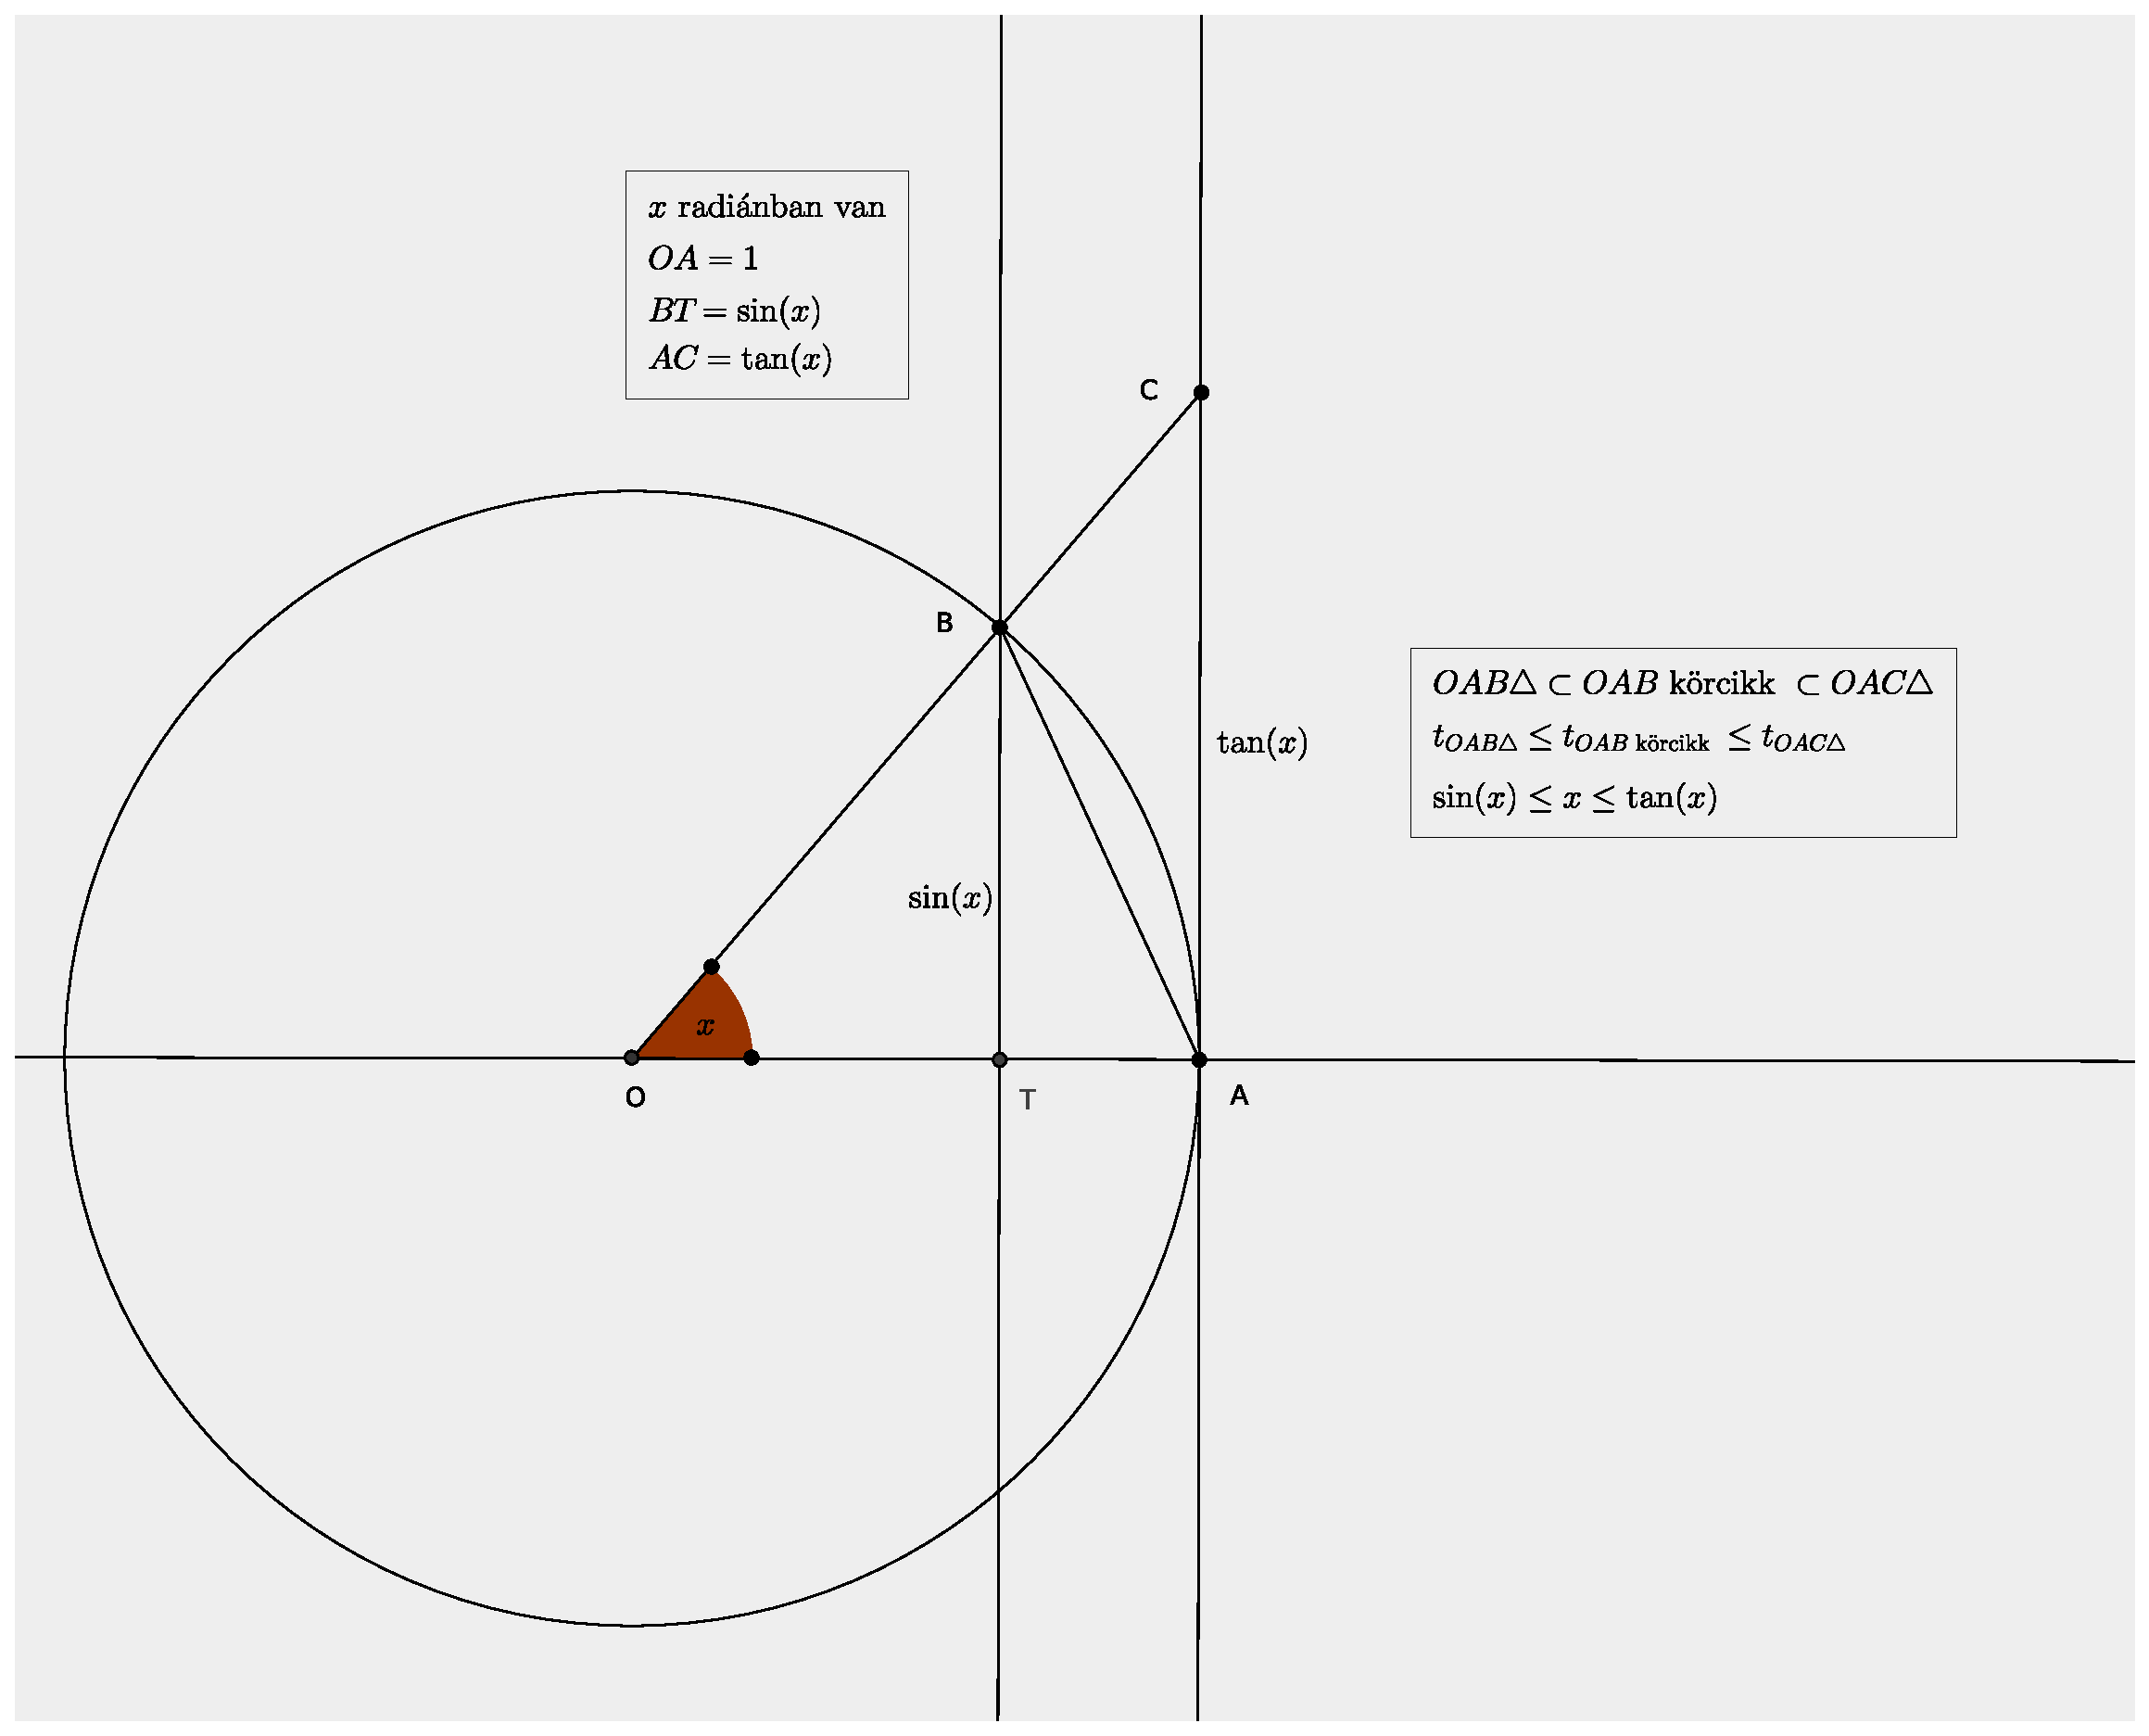
\includegraphics[width=\textwidth]{DB/fig/sin}}
%\end{center}
%\frame{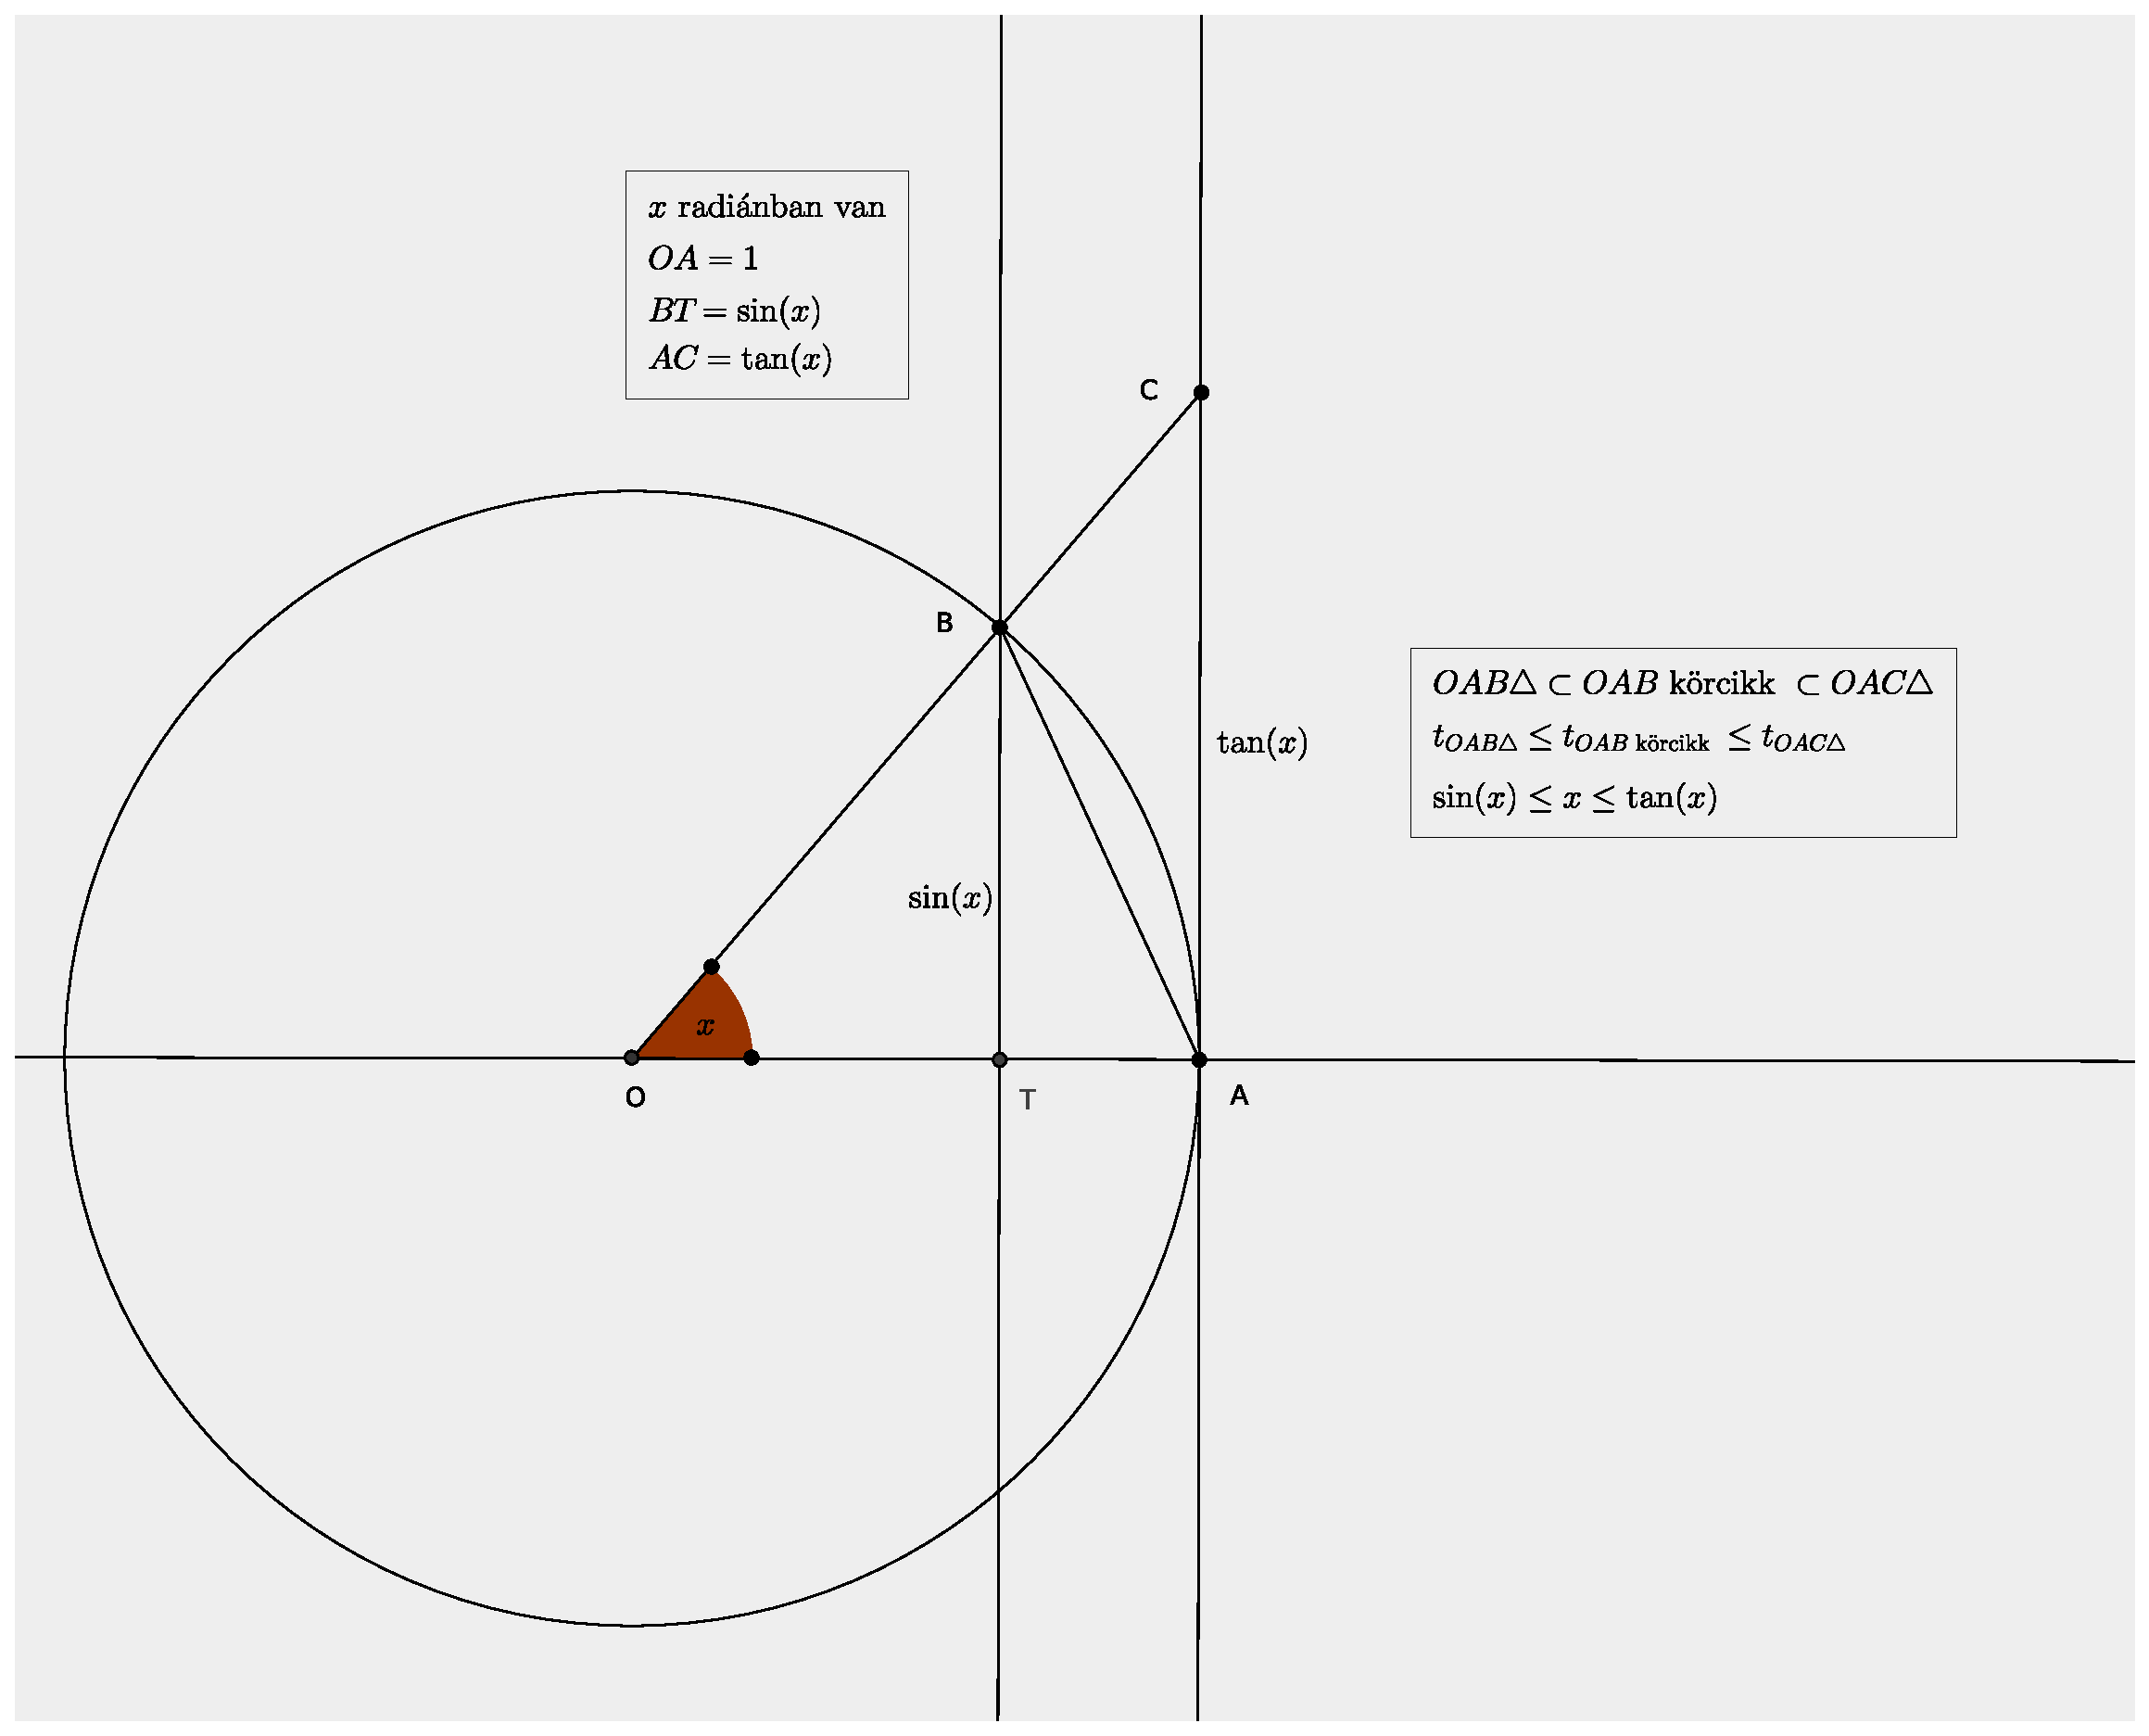
\includegraphics[scale=\textwidth]{DB/fig/sin}}
A \ref{sin-tan} lemma miatt:
\Mat{
   \cos(x)< \frac{\sin(x)}{x}< 1 \hspace{1cm} -\frac{\pi}{2}<x<\frac{\pi}{2}
}


}
\vspace{0.5cm}
\LINK{
\nameref{DBsin1}
\hfill\nameref{DBsin}
}
\newpage
\section*{\mtit{Fa}$\frac{1-\cos(x)}{x}\to 0$} \label{DBsin2}
\Fa{
\Mat{
   \lim_{h\to 0} \frac{1-\cos(x)}{x}=0
}
}
\vspace{0.5cm}
\LINK{
\nameref{DBsin2Mo}
\hfill\nameref{DBsin}
}
\newpage
\section*{\mtit{Mo}$\frac{1-\cos(x)}{x}\to 0$} \label{DBsin2Mo}
\Mo{
\Mat{
   \cos(x)=1-2\sin^2 \gzjel{\frac{x}{2}}\\
   1-\cos(x)=2\sin^2 \gzjel{\frac{x}{2}}\\
   \frac{1-\cos(x)}{x}=\gzjel{ \frac{\sin(\frac{x}{2})}{\frac{x}{2}}}^2\frac{x}{2}
}
}
\vspace{0.5cm}
\LINK{
\nameref{DBsin2}
\hfill\nameref{DBsin}
}
\newpage
\section*{\mtit{Fa}$\frac{\tg(x)-x}{x^2}\to 0$} \label{DBsin3}
\Fa{
\Mat{
   \lim_{x\to 0} \frac{\tg(x)-x}{ x^2} = 0
}
}
\vspace{0.5cm}
\LINK{
\nameref{DBsin3Mo}
\hfill\nameref{DBsin}
}
\newpage
\section*{\mtit{Mo}$\frac{\tg(x)-x}{x^2}\to 0$} \label{DBsin3Mo}
\Mo{
\Mat{
   \frac{\tg(x)-x}{ x^2}=\\
   \frac{\frac{\sin(x)}{x}\frac{1}{\cos(x)}-1}{x}=\\
   \frac{\frac{\sin(x)}{x}\frac{1}{\cos(x)}-
   \frac{\sin(x)}{x}+\frac{\sin(x)}{x}-1
   }{x}=\\
}

}
\vspace{0.5cm}
\LINK{
\nameref{DBsin3}
\hfill\nameref{DBsin}
}
\newpage

\end{spacing}
\end{document}

